\documentclass[border=8pt]{standalone}
\usepackage[T1]{fontenc}
\usepackage[utf8]{inputenc}
\usepackage{pgfplots}
\pgfplotsset{compat=1.18}
\usepackage{xcolor}

\definecolor{barcolor}{HTML}{D4940A}

\begin{document}
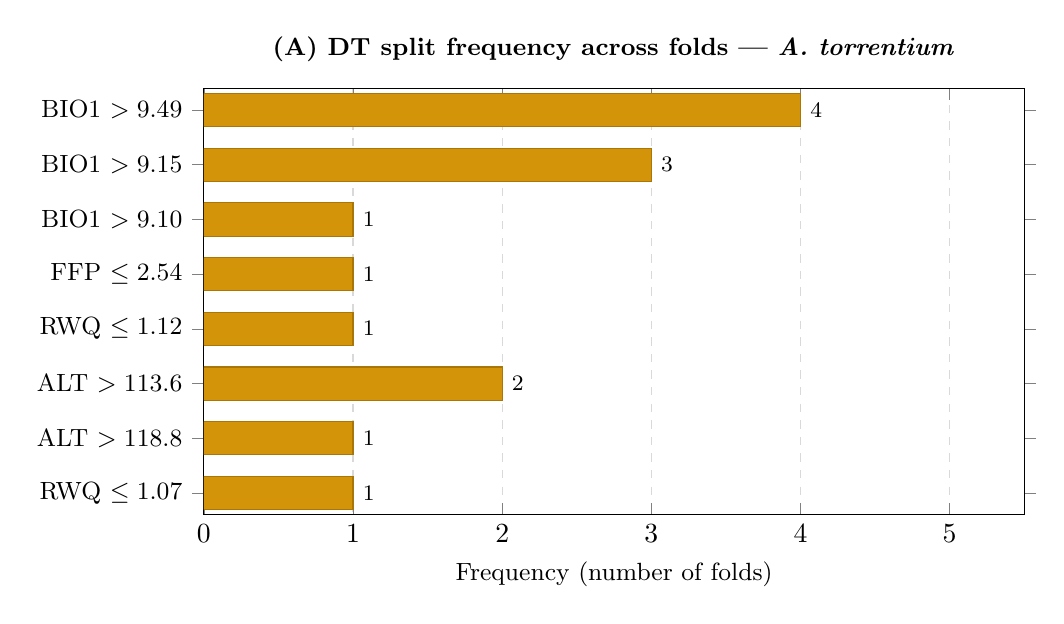
\begin{tikzpicture}
\begin{axis}[
  width=12cm, height=7cm,
  title={(A) DT split frequency across folds --- \textit{A.~torrentium}},
  title style={font=\bfseries\small},
  xlabel={Frequency (number of folds)},
  xlabel style={font=\small},
  xbar,
  bar width=12pt,
  xmin=0, xmax=5.5,
  xtick={0,1,2,3,4,5},
  ytick=data,
  yticklabels={
    {BIO1 $> 9.49$},
    {BIO1 $> 9.15$},
    {BIO1 $> 9.10$},
    {FFP $\leq 2.54$},
    {RWQ $\leq 1.12$},
    {ALT $> 113.6$},
    {ALT $> 118.8$},
    {RWQ $\leq 1.07$}
  },
  yticklabel style={font=\small},
  y dir=reverse,
  nodes near coords,
  nodes near coords style={font=\footnotesize, anchor=west},
  xmajorgrids=true,
  grid style={dashed, gray!30},
  enlarge y limits={abs=0.4},
]
\addplot[fill=barcolor, draw=barcolor!80!black] coordinates {
  (4, 0)
  (3, 1)
  (1, 2)
  (1, 3)
  (1, 4)
  (2, 5)
  (1, 6)
  (1, 7)
};
\end{axis}
\end{tikzpicture}
\end{document}
